\section{Performance evaluation}%
\label{Performance}

\commentDaniel{%
  Some data for Adrien.%
}
\Textcite{ANOBE} proposed using a modified version of \ac{KD-HES}.

\subsection{Evaluation testbed} % (fold)
\label{sub:evaluation_testbed}



\subsubsection{Simulating user behavior} % (fold)
\label{ssub:simulating_user_behavior}


To evaluate \name, we take interest in users owning a variable amount of devices of different types, and frequently switching among them.
To the best of our knowledge, there exists no real-world dataset of the devices connection times of such a user.
We have thus implemented an evaluation testbed where each user's behavior is simulated  according to the following properties:
\begin{itemize}
	\item The user owns a variable amount of devices (3 to 10). We consider the following device types: mobile (e.g. tablet, phone), portable (laptop), fixed (workstation, home computer) and server (such as a NAS, Raspberry Pi or rented appliance);
	\item She can travel between different locations, say her home, her workplace and and outside;
	\item She makes a different use of her devices depending on her location: her home computer will only be accessed at home, while her phone can be accessed everywhere (though she tends to use it the most at home, for instance).
\end{itemize}

We thus model each user with a Hidden Markov Model, as presented in section~\ref{sub:a_model_of_the_user_s_behavior}.
We keep the different possible locations $\mathcal{L}$ to a number of three, and generate different state transition matrices $A$ and emission probability matrices $B$ for each user. 

$B_{*, d}$, the probability that device $d$ is used in each location, depends on $d$'s device type: 
\begin{itemize}
	\item for each location, every mobile device $d_m$ has a random but high probability of being online: $\forall l \in \mathcal{L}, B_{l, d_m} \in [0.6, 1]$;
	\item a portable device $d_p$ has a much lower probability of being used ($\forall l \in \mathcal{L}, B_{l, d_p} \in [0.2, 0.8]$); 
	\item a fixed appliance $d_f$ has a non-zero probability of usage in only one location: $\exists l \in \mathcal{L}, \forall l' \neq l, B_{l, d_f} \in [0.4, 0.8] \& B_{l, d_f} = 0$
	\item a server $d_s$ has a very high probability of working, whatever the user's location: $\exists p \in [0.9, 1], \forall l \in \mathcal{L}, B{l, d_s} = p$.
\end{itemize} 

\begin{figure}[t]
\centering
\vspace{-1em}

$$A =
\kbordermatrix{
      & W            & O            & H            \cr
    W & \sfrac{2}{3} & \sfrac{1}{3} & 0            \cr
    O & \sfrac{1}{3} & \sfrac{1}{3} & \sfrac{1}{3} \cr
    H & 0            & \sfrac{1}{3} & \sfrac{2}{3} \\[0.3em]
}, \;
B = 
\kbordermatrix{
      & W     & O   & H   \cr
    p & 0.7 & 0.6 & 0.8 \cr
    w & 0.7 & 0   & 0   \cr
    h & 0   & 0   & 0.7 \cr
    l & 0.2 & 0.4 & 0.6 \\[0.3em]
}$$

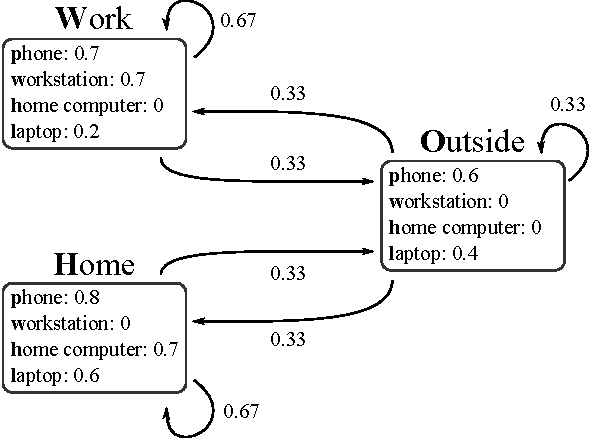
\includegraphics[width=0.9\columnwidth]{figures/hmm.pdf}
\caption{ \label{fig:hmm} Example Hidden Markov Model (HMM) of a user's behavior.}
\end{figure}



\begin{figure}[t]
\centering
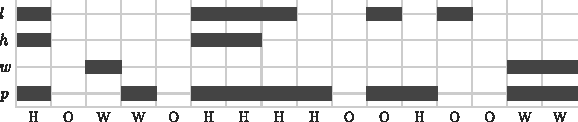
\includegraphics[width=\columnwidth]{figures/sample_usage.pdf}

\caption{\label{fig:sample_usage}Sample device usages using the previous HMM specifications. 
%The bottom line reads the HMM's states: \textbf{W}ork, \textbf{O}utside, and \textbf{H}ome, while the dark lines read when the devices (\textbf{h}ome computer, \textbf{p}hone, and \textbf{w}orkstation) are online.
}

\end{figure}

% subsubsection simulating_user_behavior (end)

% subsection evaluation_testbed (end)